\section{Framework Design}

\begin{concept}{Framework Grundlagen}
Ein Framework ist ein Programmiergerüst mit folgenden Eigenschaften:
\begin{itemize}
    \item Bietet wiederverwendbare Funktionalität
    \item Definiert Erweiterungs- und Anpassungspunkte
    \item Verwendet Design Patterns
    \item Enthält keinen applikationsspezifischen Code
    \item Gibt Rahmen für anwendungsspezifischen Code vor
    \item Klassen arbeiten eng zusammen (vs. reine Bibliothek)
\end{itemize}
\end{concept}

\subsection{Design Patterns in Frameworks}

\begin{definition}{Factory Method}
\textbf{Problem:} Flexible Objekterzeugung in wiederverwendbarer Klasse

\textbf{Lösung:}
\begin{itemize}
    \item Abstrakte Factory-Methode in Creator-Klasse
    \item Konkrete Subklassen überschreiben Methode
    \item Parallele Vererbungshierarchien
\end{itemize}

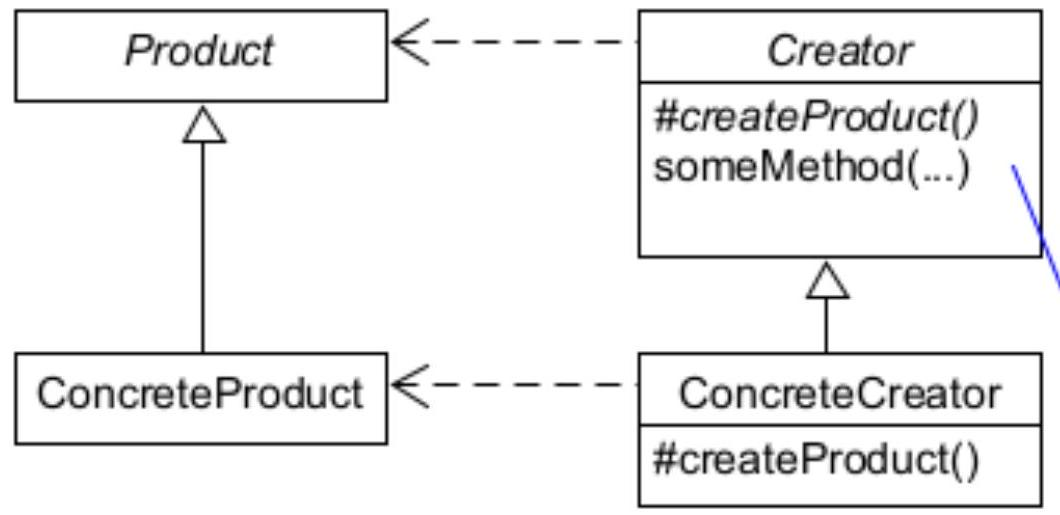
\includegraphics[width=0.6\linewidth]{images/2025_01_02_73d93f10fa91ab6123dcg-16}
\end{definition}

\begin{definition}{Abstract Factory}
\textbf{Problem:} Erzeugung zusammengehörender Objekte ohne Kenntnis konkreter Klassen

\textbf{Lösung:}
\begin{itemize}
    \item AbstractFactory-Interface definieren
    \item Pro Produkt eine create-Methode
    \item Konkrete Factories implementieren Interface
\end{itemize}
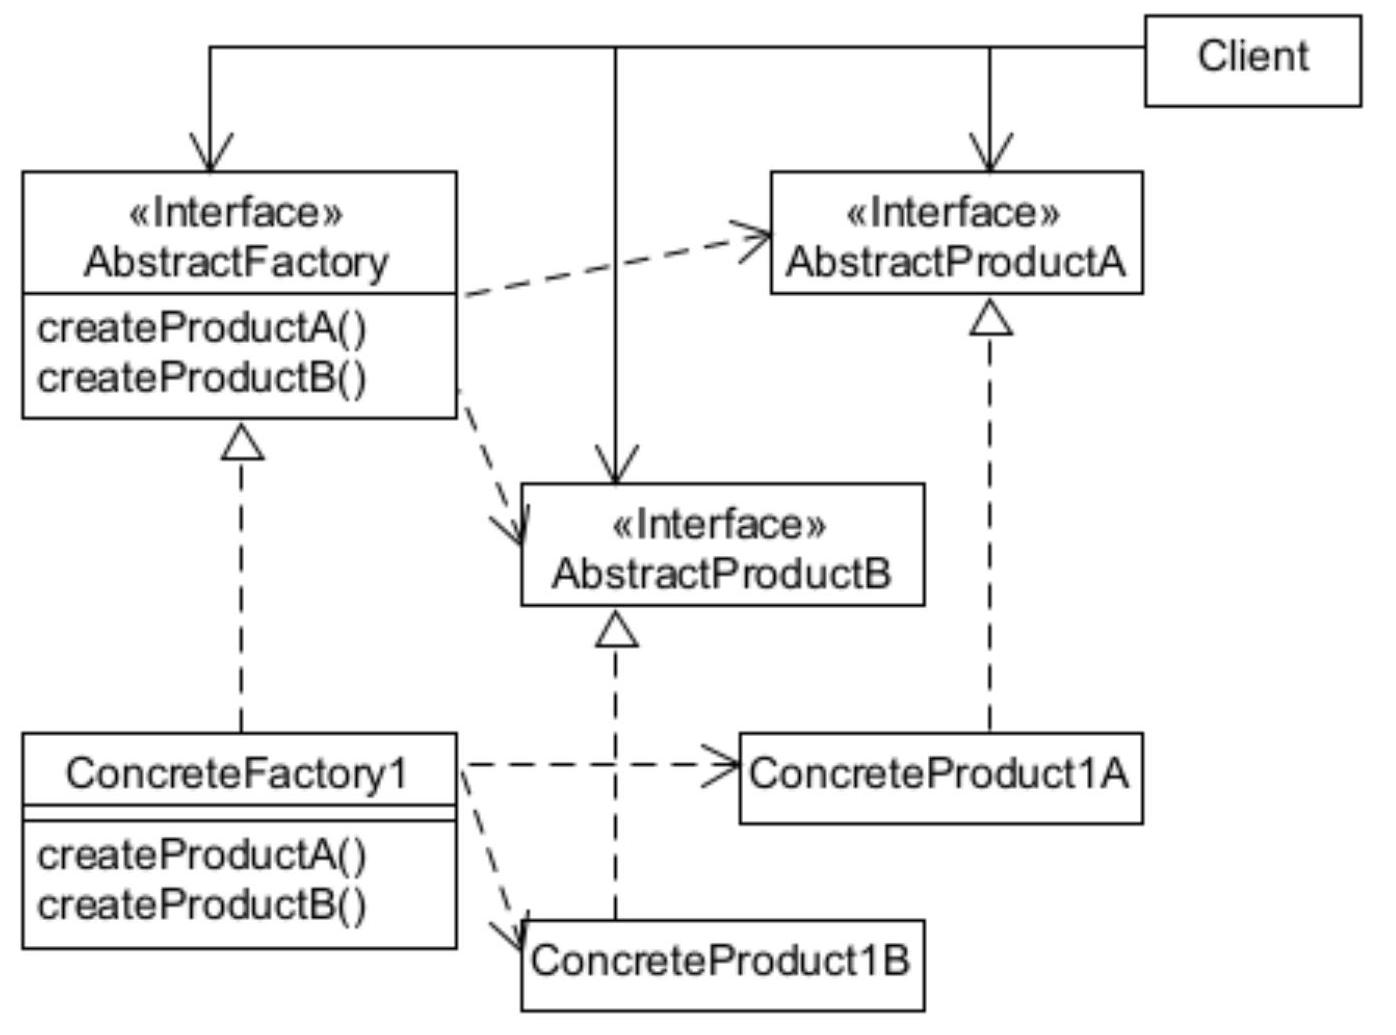
\includegraphics[width=0.8\linewidth]{images/2025_01_02_73d93f10fa91ab6123dcg-13}
\end{definition}

\begin{definition}{Template Method}
\textbf{Problem:} Algorithmus mit anpassbaren Teilschritten

\textbf{Lösung:}
\begin{itemize}
    \item Template Method in abstrakter Klasse
    \item Hook-Methoden für variable Teile
    \item Hollywood Principle: "Don't call us, we'll call you"
\end{itemize}
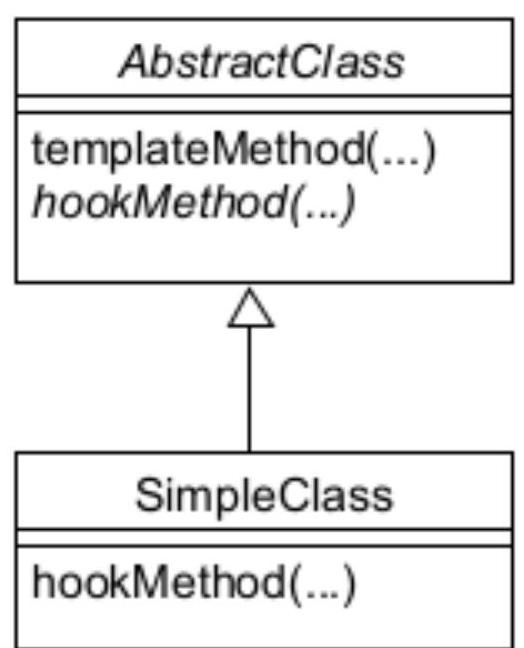
\includegraphics[width=0.3\linewidth]{images/2025_01_02_73d93f10fa91ab6123dcg-22}
\end{definition}

\subsection{Moderne Framework Mechanismen}

\begin{definition}{Annotation-basierte Konfiguration}
Moderne Frameworks nutzen Annotationen für:
\begin{itemize}
    \item Dependency Injection
    \item Konfiguration
    \item Interface-Implementation
    \item Funktionalitätserweiterung
\end{itemize}

\textbf{Vorteile:}
\begin{itemize}
    \item Keine harte Abhängigkeit zum Framework
    \item Deklarativer Programmierstil
    \item Reduzierung von Boilerplate-Code
\end{itemize}
\end{definition}

\begin{concept}{Annotations als Steuerungsmechanismus}
\textbf{Auswertung von Annotationen:}
\begin{itemize}
    \item Framework wird mit Anwendung gestartet
    \item Sucht Anwendungsklassen auf dem Klassenpfad
    \item Untersucht Annotationen
\end{itemize}

\textbf{Mögliche Framework-Aktionen:}
\begin{itemize}
    \item Dependency Injection in Anwendungsobjekte
    \item Automatische Interface-Implementierung
    \item Funktionalität zu Klassen hinzufügen
\end{itemize}
\end{concept}

\begin{concept}{Aspekt-orientierte Programmierung}
\textbf{Querschnittliche Belange:}
\begin{itemize}
    \item Logging
    \item Sicherheit
    \item Transaktionsmanagement
    \item Performance Monitoring
\end{itemize}

\textbf{Implementation mit Annotations:}
\begin{itemize}
    \item Aspekte definieren
    \item Join Points festlegen
    \item Advice implementieren
\end{itemize}
\end{concept}

\begin{KR}{Framework Design Principles}
\textbf{1. Abstraktionsebenen definieren}
\begin{itemize}
    \item Core API
    \item Extensions
    \item Standard-Implementierungen
\end{itemize}

\textbf{2. Erweiterungsmechanismen}
\begin{itemize}
    \item Interface-basiert
    \item Annotations
    \item Composition
\end{itemize}

\textbf{3. Qualitätskriterien}
\begin{itemize}
    \item Usability der API
    \item Flexibilität
    \item Wartbarkeit
\end{itemize}
\end{KR}

\begin{KR}{Framework-Extensions entwickeln}
\textbf{1. Extension Points identifizieren}
\begin{itemize}
    \item Core-Funktionalität analysieren
    \item Variationspunkte bestimmen
    \item Interface-Hierarchie planen
\end{itemize}

\textbf{2. Extension Mechanismen}
\begin{itemize}
    \item Interface-basiert
    \item Annotation-basiert
    \item Discovery Mechanism implementieren
\end{itemize}
\end{KR}

\subsection{Framework Integration und Testing}

\begin{KR}{Framework Integration}
\textbf{1. Convention over Configuration}
\begin{itemize}
    \item Namenskonventionen einhalten
    \item Standard-Verhalten nutzen
    \item Nur Ausnahmen konfigurieren
\end{itemize}

\textbf{2. Dependency Injection}
\begin{itemize}
    \item Abhängigkeiten deklarieren
    \item Framework übernimmt Injection
    \item Constructor- oder Setter-Injection
\end{itemize}

\textbf{3. Interface-basierte Entwicklung}
\begin{itemize}
    \item Interfaces definieren
    \item Framework generiert Implementation
    \item Methodennamen als Spezifikation
\end{itemize}
\end{KR}

%todo: Add examples for:
% - Framework extension implementation
% - Annotation processing
% - AOP implementation
% - Integration patterns